\documentclass[../../main.tex]{subfiles}

\graphicspath{{\subfix{../../immagini/}}}

\begin{document}

I metodi introdotti negli scorsi paragrafi, come già accennato, risultano in molti contesti fortemente limitati nel tipo di pattern che possono descrivere, per questo motivo si rendono necessari modelli più \textit{espressivi} per poter approssimare le funzioni più complesse.

Introduco quindi ora il concetto di \textbf{rete neurale artificiale} e mi concentro poi su due specifiche \textit{architetture} di reti: \textit{percettroni multistrato} e \textit{reti ricorrenti}, che saranno quelle utilizzate negli esperimenti descritti nei capitoli successivi.  

Citando \cite{kriesel2007bin}:

\begin{dfn}
    Una \textbf{rete neurale} è una tripla $(N, V, w)$ dove $N$ rappresenta l'insieme di neuroni della rete, $V$ è un insieme della forma $\{(i, j) \ | \ i,j \in \mathbb{N} \}$ e rappresenta le \textbf{connessioni} tra le unità della rete $i$ e $j$, infine $w$ è una funzione definita come:
    \[w : V \rightarrow \mathbb{R}\]
    che ritorna il \textbf{peso} di una connessione $(i, j)$
\end{dfn}

Una rete è quindi formata da unità computazionali, dette \textbf{neuroni}, collegate tra loro da \textit{connessioni} caratterizzate da un \textit{peso}, che intuitivamente rappresentano la forza di una connessione.

\begin{figure}[H]
    \centering
    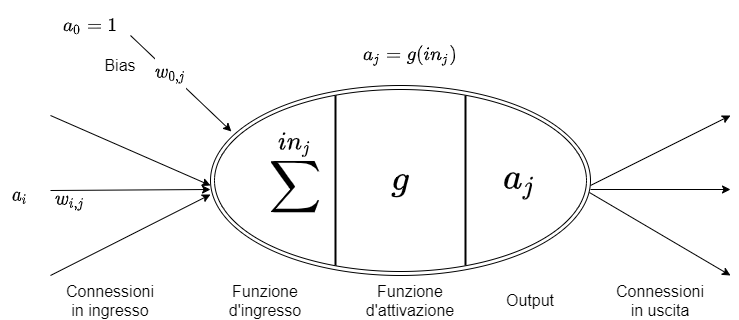
\includegraphics[width=\textwidth]{immagini/4_2/neuron.png}
    \caption{Struttura di un neurone}
    \label{fig:neuron}
\end{figure}

Ogni neurone risulta collegato con una serie di altri neuroni ricevendo in ingresso i rispettivi output che trasforma in base al valore dei relativi pesi $w_{i,j}$, una volta prodotto l'output questo viene a sua volta \textit{propagato} ad una serie di altre unità funzionali.

Formalmente posso suddividere la struttura di un neurone in diverse parti (Figura \ref{fig:neuron}): ogni valore ricevuto in ingresso prende il nome di \textbf{attivazione} $a_i$, questi vengono prima passati attraverso una funzione d'ingresso, che spesso viene definita come somma \textit{pesata} dei valori d'ingresso:
\[in_j = \sum_{i=0}^n {w_{i,j} a_i}\]
Il risultato della funzione d'ingresso viene poi dato in input alla \textit{funzione d'attivazione} $g$:
\[a_j = g(in_j) = \sum_{i=0}^n {w_{i,j} a_i}\]
Infine il valore d'attivazione viene passato attraverso una \textit{funzione di output} che spesso semplicemente corrisponde ad una funzione identità:
\[f_{out}(a_j) = a_j\]
In generale la funzione d'attivazione può avere diverse forme:

\begin{figure}[H]
    \centering
    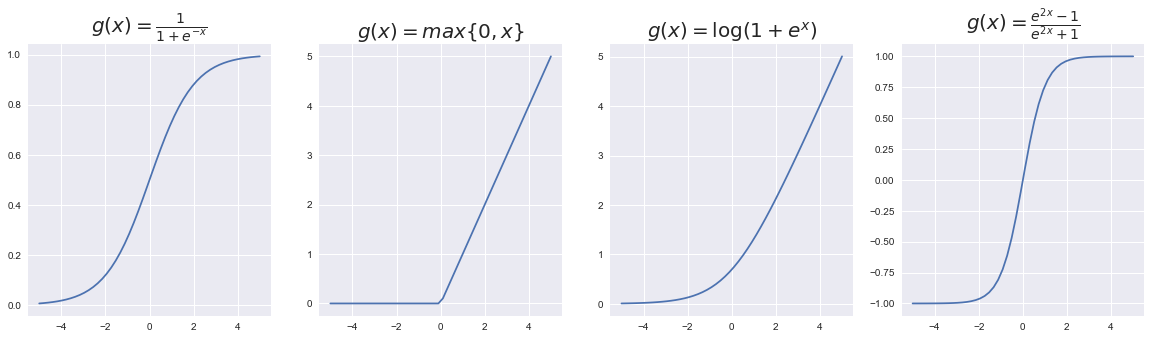
\includegraphics[width=\textwidth]{immagini/4_2/activation_func.png}
    \caption{Esempi di tipiche funzioni d'attivazione}
    \label{fig:activations}
\end{figure}

È importante che una funzione d'attivazione sia:
\begin{itemize}
    \item \textbf{Non lineare}: altrimenti l’uscita della rete sarebbe sempre lineare e il modello sarebbe troppo semplice.
    \item \textbf{Differenziabile}: su buona parte del dominio e monotona non decrescente, per poter facilitare la applicazione di algoritmi basati sulla discesa del gradiente.
\end{itemize}
Nel caso in cui $g$ sia una funzione a soglia (Figura \ref{fig:threshold}) parlo di \textbf{percettrone}.

Una volta definita la struttura di un neurone è utile analizzare il come questi neuroni si connettono per andare a formare la rete: le due tipologie di \textit{architetture} utilizzate negli esperimenti sono la \textbf{rete feed forward} (Figura \ref{fig:feedforward}) e la \textbf{rete ricorrente}:

\begin{dfn}
    Una \textbf{rete feedforward} è composta da un livello d'ingresso e da un livello d'uscita e da uno o più livelli nascosti. Le connessioni in questa topologia sono permesse solo tra neuroni di livelli consecutivi.
\end{dfn}

È importante sottolineare che se il numero di livelli nascosti è superiore a 3 si parla di \textbf{reti profonde}.

\begin{dfn}
    Una \textbf{rete ricorrente} è un topologia in cui sono permesse connessioni tra neuroni che generano ricorrenza: parlo nello specifico di ricorrenza \textbf{diretta} nel caso in cui un neurone sia connesso con sé stesso, mentre parlo di ricorrenza \textbf{indiretta} quando sono ammesse connessioni verso livelli precedenti, in quest'ultimo caso una ipotetica unità $i$ potrebbe auto-influenzarsi propagando la propria attivazione al neurone successivo $i$ che a sua volta propaga il proprio output verso il livello d'ingresso.
\end{dfn}

A differenza quindi di ciò che accade con una topologia feedforward, nel caso di una rete ricorrente il risultato ad un determinato input può essere funzione degli input precedenti, reti che sfruttano questa architettura quindi supportano meccanismi di "\textit{memoria a breve termine}", ciò li rende modelli più interessanti per alcuni problemi, ma ovviamente anche più complessi.

\begin{figure}[H]
    \centering
    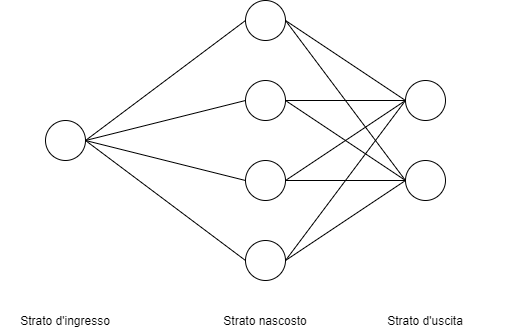
\includegraphics[width=\textwidth]{immagini/4_2/feed_forward.png}
    \caption{Esempio di rete neurale con architettura feed forward}
    \label{fig:feedforward}
\end{figure}



\end{document} 